% !TeX root = ../Main.tex

\chapter{Basics}
\label{ch:basics}
In this chapter, the two most important technologies for the framework are explained. This is necessary to get an understanding of the technical difficulties it faces and how the underlying concepts work. First, in Section~\ref{sec:uima} \uima{} is introduced. After an in-depth introduction into the framework originally designed by IBM, \uimafit{} will be explained. \uimafit{} builds on top of \uima{}, providing the developer with a native Java interface for creating and instantiating plug-ins. Strongly related to the framework introduced in Chapter~\ref{ch:implementation} are the two native scaling frameworks \uimacpe{} and \uimaas{}. 


The second section of this chapter will be about \spark{}. While no advanced knowledge is needed to comprehend the usage of \spark{} as a distributed computation framework, it will still be a substantial part of the \uima{} scaling framework in Chapter~\ref{ch:implementation}. Thus, a rather superficial overview of its structure and distribution algorithm will be given. Although it was not used in the development of the framework, \docker{} will be introduced, since it was heavily utilized in the evaluation described in Chapter~\ref{ch:evaluation}.

Since numerous attempts have been made, scaling \uima{} in different settings, with varying implementation requirements, some related work will be presented in Section~\ref{sec:related}, namely Leo, providing a native Java interface for \uimaas{}, and v3NLP, a framework especially designed for usage in a medical environment and with plug-ins of such sort. Although most important aspects and concepts of \uima{} are also defined in the specifications, some minor changes and additions were made in the implementations. Since the framework must handle the actual implementation, all the presented concepts will be taken from Apache \uima{} instead of the \uima{} specification of 2009.



\section{UIMA-Family}
\label{sec:uima}
Unstructured Information Management Architecture (UIMA) Version 1.0 itself is an \oasis{} standard from 2009\footurl{http://docs.oasis-open.org/uima/v1.0/uima-v1.0.html}{2018-09-03} that defines an interface for software components, or plug-ins, which are called analytics. Those analytics are supposed to analyze unstructured information and assign machine readable semantics to it. The standard also defines ways to represent and interchange this data between analytics in favor of interoperability and platform-independence. 

Apache \uima{} is the open-source implementation of said \uima{} specification. A common problem with Apache \uima{} is scaling \cite{divita2015scaling,epstein2012making,ramakrishnan2010building}. It  provides two distinct interfaces to analyze larger collections of unstructured data itself, with one being \uimaas{} and the other being the more dated and less flexible \cpe{} \cite{OASIS:UIMA:2009}.
Apache \uima{} is available for Java and C++, while its scaling solutions, \uimacpe{} and \uimaas{} are only available for Java, which is why this thesis focuses on the Java implementation. Since \uima{} and Apache \uima{} have very similar names, which may lead to confusion, it is common practice to call the implementation simply \uima{} and explicitly state when talking about the specification. This practice will be adopted for the rest of the thesis.



\subsection{Apache UIMA}

Apache \uima{} is one of few general approaches to implement \nlp{} solutions and the only commonly known implementation of the specification with the same name. With a very modular architecture, \uima{} is a popular tool that can be applied to a majority of \nlp{} problems. A large part of the popularity of \uima{} stems from the large \dkpro{} collection of components, containing hundreds of analysis modules and precomputed language models \cite{eckartdecastilho-gurevych:2014:OIAF4HLT}, which can be imported into existing Java projects with the build automation tool Apache Maven \cite{dkpro}.

\uima{} is usually used to process not a single but whole corpora of documents. A document in this sense is text, although the \uima{} specification permits other data types as well. However, \uima{} can not yet handle other data types without serializing it first. The \uima{} specification, as well as the implementation do not directly pose limitations to the document size but since documents are stored in native Java String variables, which themselves are implemented as arrays of chars, the practical limit of documents sizes is dependent on the \jvm{} version and is around one to two gigabytes \cite{so:javastrings} per document. In the context of \uima{}, such a document is called a \sofa{}.

An analytic in the \uima{} specification is called an \emph{Analysis Engine} in the implementation. For the most part, an \anen{} is code, that gets an input \cas{} and produces a number of analysis results on the \sofa{}. Common examples for \anens{} are Segmentation, Tokenization, and Part-of-Speech finding algorithms \cite{dkpro}. However, since an \anen{} contains arbitrary Java code, any form of analysis can be instrumentalized by \uima{}. It is defined by an \xml{} Analysis Engine descriptor. Such an \anen{} can either be a so-called \emph{primitive} or an \emph{aggregate} engine. An aggregate engine simply contains one or more other \anens{}, that are aggregated into one single engine.

Analysis results are stored as annotations. An annotation has at least two attributes \lstinline[language=Java]|int begin| and \lstinline[language=Java]|int end|, indicating the start and end index of the \sofa{}s substring this annotation is associated with. This concept is theoretically extendable to any kind of \sofa{} that contains any sort of subsets, for example images or audio and video streams. However, this is impractical for reasons mentioned above. It is possible, but uncommon, to define other types of subsets on a string that -- for example -- permit multiple segments. Such subsets can be implemented in a custom implementation of the \lstinline|AnnotationBase| class, which in turn may omit the concept of a \lstinline|begin| and \lstinline|end|. Since an important reason of the popularity of \uima{} is due to the large \anen{} repositories and the possibility to reuse already published code, custom annotation implementations are rarely used because it would most likely lead to incompatibilities. However, subclassing the \lstinline|Annotation| class is often done to ensure type safety. Building such an annotation hierarchy leads to the creation of a Type System.

The Type System is a schema of all available types of annotations that may be associated with a current \sofa{}, thus it provides the meta data for the annotations. It is defined by an \xml{} Type System descriptor that is usually used by the \emph{JCasGen}, a Java code generator for \uima{} types. On creation, a parent Type System can be specified, allowing inheriting from types that are not defined in the current context and encapsulate all in a single larger Type System.

The \sofa{}, all analysis results in form of annotations that are compliant to an underlying Type System, and the Type System itself are stored together in one wrapping object, called a \cas{}. It is the sole input an \anen{} gets, since it incorporates the complete context needed for the analysis. To store annotations efficiently, different indexes are created, providing fast access to commonly used queries like overlapping or distinct annotations. Furthermore, a \cas{} object provides different Views, lightweight versions of a \cas{}, that store their own \sofa{} and annotation index. These Views are identified by a String, while the original data of the \cas{} is usually called the \emph{Initial View}.

A \emph{Collection Reader} implements an interface very similar to the well-known \lstinline|Iterator|, namely it provides the functions \lstinline|boolean hasNext()| and \lstinline|CAS getNext()|. A Collection Reader usually takes the role of initializing the \cas{} with the \sofa{}. Well known Collection Readers achieve this by reading from a file system, a database or \lstinline|Collection| object, but any other collection may be read by implementing a custom Collection Reader. It is also configured by writing an \xml{} descriptor file.

Multiple Analysis Engines that form a complete flow of analysis are commonly known as a \emph{pipeline}. Since multiple \anens{} can be aggregated into one, a pipeline is usually an instance of a single aggregate Analysis Engine. Sometimes a pipeline is meant to also include a Collection Reader, however this will not be the case in this thesis. Because of the convention to call analysis results annotations, \anens{} are often called \emph{Annotators}, which is not correct in general, since engines do not need to attach any annotations to the input \cas{}.

\begin{figure}[hbt]
	\centering
	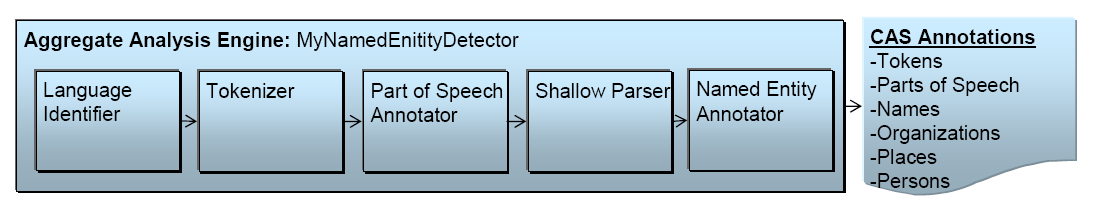
\includegraphics[width=1\textwidth]{uima-pipeline}
	\caption[An example UIMA pipeline for NER.]{An example \uima{} pipeline for named entity recognition \cite{uimasdk}.}
	\label{fig:uimaner}
\end{figure}

Figure~\ref{fig:uimaner} shows a simplified view of an analysis pipeline for named entity recognition. Given a \cas{} by a Collection Reader (omitted here), the pipeline which is really just a aggregate Analysis Engine starts to identify the language of the text with an Analysis Engine specifically designed to do exactly this. This \anen{} stores the results inside the \cas{} and forwards it to the next engine in line, which is a tokenizer. 

A tokenizer annotates words, sentences and punctuation and is highly language dependent. It uses the analysis result given by the \anen{} before deciding upon an algorithm or model to use according to the detected language. After tokenization, a Part-Of-Speech Tagger annotates each words part of speech with a different annotation according to a tag set. There are a number of tag sets for most languages, as for example the Penn Treebank Project tag set\footurl{https://www.ling.upenn.edu/courses/Fall_2003/ling001/penn_treebank_pos.html}{2018-09-08} for English and the \stts{} for German. The Part-Of-Speech Tagger is highly language dependent because of this. It also utilizes the results of the tokenizer, since it iterates over all annotations that are words (as opposed to annotations that span punctuation).

Afterwards the \cas{} gets put into a Shallow Parser, which analyzes Part-Of-Speech tags and their semantic relation among other tags in the same sentence. In a sentence `I like green apples.' a Part-Of-Speech Tagger would correctly decide that `green' is an adjective and `apples' is a noun. However, a parser would combine those two to form `green apples', a Noun Phrase, because `green' is an adjectival modifier of `apples'. A Parser may also be used to improve the results of a previous Part-Of-Speech tagging.

A Named Entity Recognizer then takes the \cas{} object and looks for fitting entities. This is commonly an entry of a given noun list, but can be more sophisticated, depending on the wanted precision, the entity type and computation speed. After the last part of the pipeline returns, the analysis is done. The resulting \cas{} now includes a number of analysis results in form of annotations which can now be extracted or processed further.

\subsection{UIMAfit}
\label{ssec:uimafit}
Since \uima{} needs \xml{} descriptor files to configure and describe most of its components, especially pipelines and type systems, developing in it is very \xml{} heavy and leads to code that is hard to maintain. Apache \uimafit{} is a framework that builds on \uima{}, providing an interface to programmatically describe, instantiate, and deploy \uima{} components \cite{ogren-bethard:2009:SETQA-NLP}. \uimafit{} also provides an interface to dynamically write \xml{} descriptor files for \uima{} components. However, since it is able to instantiate and deploy said components without the need of \xml{} files, those are mostly ignored. \uimaas{}, a native \uima{} scaling framework described in Section~\ref{ssec:uimaas}, is known to be widely incompatible with \uimafit{}, which is what led to the creation of Leo, described in Section~\ref{ssec:leo}.

\uimafit{} has been part of the Apache \uima{} project since 2012 and is therefore officially supported \cite{github:uimafit}. 



\subsection{UIMA-CPE}
\label{ssec:uimacpe}
\uimacpe{} was the first method to add distributed computation capability to \uima{}. Nowadays it has been replaced by \uimaas{} and is mostly obsolete. It made use of so called \emph{\cas{} Consumers}, engines that do not analyze the \cas{}, but extract the needed analysis results from it and process the data as wanted. Common uses for \cas{} Consumers are writing analysis results into a database or serializing the whole \cas{} into a \xmi{} file. \cas{} Consumers have been deprecated and replaced by \anens{} since 2006, mainly because \cas{} Consumers do not provide any new functionality or are semantically different from Analysis Engines. Historically a \cas{} Consumer would not modify a \cas{} object. This convention of a reading-only and consuming Analysis Engine is often used to provide maximum modularity among \uima{} engines.


Another concept exclusive to \uimacpe{} are \cas{} Initializers, which also have been deprecated for over a decade, but are still included in \uima{}. A \cas{} Initializer was responsible to populate a \cas{} from an object given by the Collection Reader. It therefore implemented the function \lstinline|initializeCas(Object document, CAS cas)|. This was used for more complex collection reading capabilities, therefore \cas{} Initializers are generally seen as a plug-in to Collection Readers to extend their functionality. If -- for example -- only table of contents of larger documents are meant to be analyzed, then a Collection Reader would read the whole document and pass it to the \cas{} Initializer, which would search for a table of contents and fill the \cas{} with its findings and discard the rest of the document.


\begin{figure}[hbt]
	
	\centering
	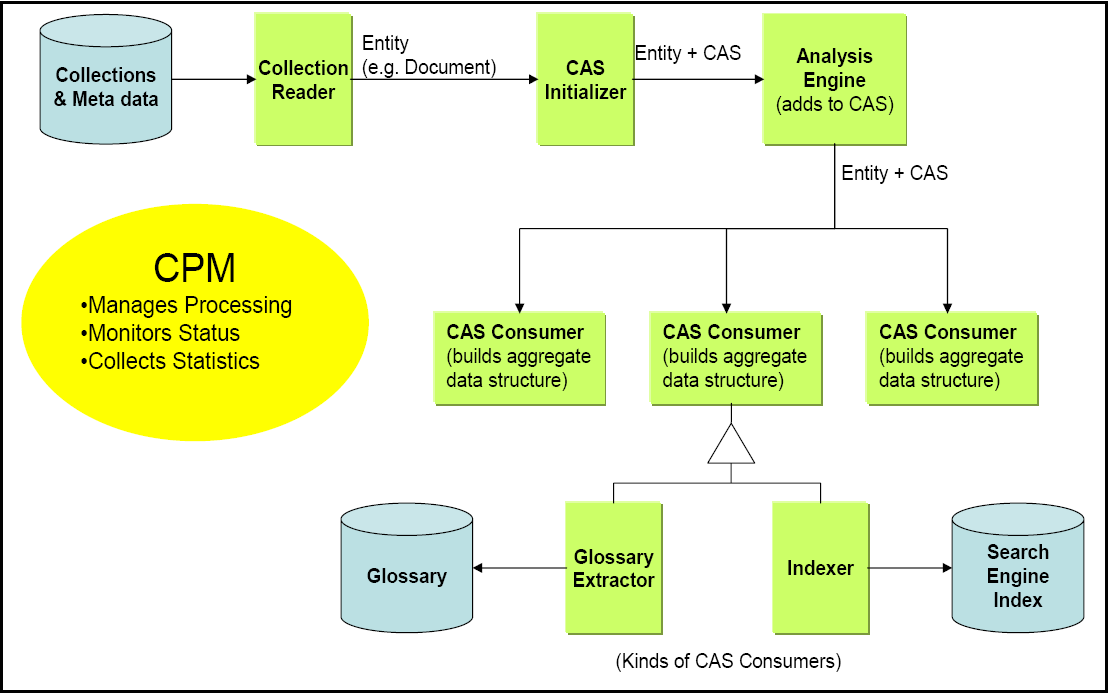
\includegraphics[width=1\textwidth]{uima-cpe}
	\caption[All \uimacpe{} components.]{All \uimacpe{} components \cite{uimacpe}.}
	\label{fig:uimacpe}
\end{figure}


Figure~\ref{fig:uimacpe} shows a complete example pipeline. It starts with any kind of collections, maybe containing meta data. A common example would be a folder hierarchy with `last modified' timestamps. The Collection Reader is aware of this collection and implements an \lstinline|Iterator| like interface, returning plain \lstinline|Object|s. These are given to the \cas{} Initializer. Notice, that the \cas{} Initializer must be aware of what kind of entity the Collection Reader sends it. The \cas{} Initializer then fills a \cas{} object with some data from the given input \lstinline|Object|. It might also create some first annotations to store meta data inside the \cas{}, such as the source document \URL{} or the creation timestamp. 

The \cas{} is then sent to the pipeline, containing one or more \anens{}, providing analysis results in form of annotations that are stored inside the \cas{}. Notice that the corresponding \cas{} object for a document always stays the same identical object. A \cas{} and its corresponding document are therefore closely associated to each other. After the analysis phase, the \cas{} is sent to the \cas{} Consumers. Those aggregate the analysis results and process it further. This process is commonly the indexing into a database or printing logs to a log file or console. Since \cas{} Consumers have read-only access to the \cas{} object they get, all of them might be processed in parallel, provided that the consumers do not interfere with each other.

All these components in combination with the \uima{} \cpm{} forms the \uimacpe{}. The Collection Processing Manager provides configuration options for deployment, instantiation, and error recovery. It monitors the whole process and collects statistics. By configuration of the \cpm{} scaling is possible either locally or on distributed machines.

For all three components introduced in this Section~\ref{ssec:uimacpe} \xml{} descriptor files are needed for configuration. The concept of a \uimacpe{} is widely incompatible with \uimafit{}, described in Section~\ref{ssec:uimafit}. \uimafit{} is able to instantiate a \cpe{}, but relies on some hardcoded default configuration, making complex multithreading applications impossible\footurl{https://uima.apache.org/d/uimafit-2.0.0/api/org/apache/uima/fit/cpe/CpeBuilder.html}{2018-09-08}.


\subsection{UIMA-AS}
\label{ssec:uimaas}
\uimaas{} is the successor of \uimacpe{}, providing more flexibility for scaling and deploying than its predecessor. It deploys \anens{} as services and registers them at a broker. \uimaas{} ships with a preconfigured instance of Apache ActiveMQ, which is an open source message broker that implements the Java Messaging Service (JMS). However, other broker implementations can also be used, but must be configured for usage with \uimaas{} and JMS. If a \uimaas{} client now queries the broker, it submits a serialized \cas{} object to the input queue that is responsible for the wanted analysis. When any registered service finishes its current job, it pulls a new \cas{} from the broker and starts processing. This analysis process can also be multithreaded inside a single service. This is configurable by the deployment \xml{} descriptor files of the \anens{}, but must be handled with care since multiple instances of Analysis Engines in the same \jvm{} share static resources. After finishing the process, either successfully or by failing, the service returns the \cas{} object to the brokers corresponding output queue where it waits until the broker finds time to forward it to the waiting client. The described process can be seen in Figure~\ref{fig:uimaas-ae}. The user-defined \anen{} get wrapped by a \uimaas{} controller, that handles communication with the input and output queue. These queues are provided by a broker, here ActiveMQ.

\begin{figure}[hbt]
	\centering
	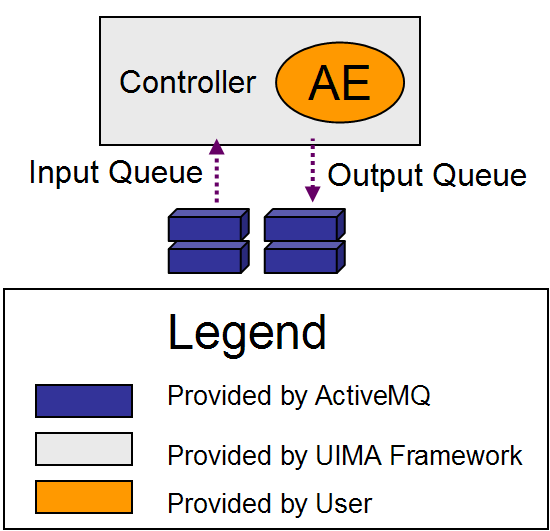
\includegraphics[width=0.5\textwidth]{uima-as-ae}
	\caption[An Analysis Engine as a service in UIMA-AS.]{An Analysis Engine as a service in \uimaas{} \cite{uimaas:documentation}.}
	\label{fig:uimaas-ae}
\end{figure}

To provide capabilities of a more complex analysis flow instead of the simple synchronous order, the user can implement what is called a \emph{Flow Controller}. An aggregate Analysis Engine can have at most one Flow Controller, that handles what \anen{} gets the \cas{} next. Usually \uima{} defaults to the \lstinline|FixedFlow| class, which executes \anens{} one after another, but more sophisticated flows can be implemented. If an aggregate Analysis Engine contains such a Flow Controller, further queues are installed. Figure~\ref{fig:uimaas-aea} shows such an advanced pipeline containing a flow controller and two delegate Analysis Engines. Submitting a \cas{} to the aggregate Analysis Engine queues it into the queue of the Flow Controller (FC). When it finishes its current computation, the Controller is faced with the decision which delegate Analysis Engine should obtain the \cas{} for processing and appends it to the corresponding queue. Notice that said queue is also provided by ActiveMQ (or any other implementation). After analysis, the \cas{} is sent back to the Flow Controller, or more specifically its output queue. It may now decide to send the processed \cas{} to another delegate \anen{} or stop processing and output it to the brokers output queue. The large amount of queue may seem excessive, but it is necessary to provide a synchronous execution of the Flow Controller and -- if configured -- the Analysis Engines without loss of data.

\begin{figure}[hbt]
	\centering
	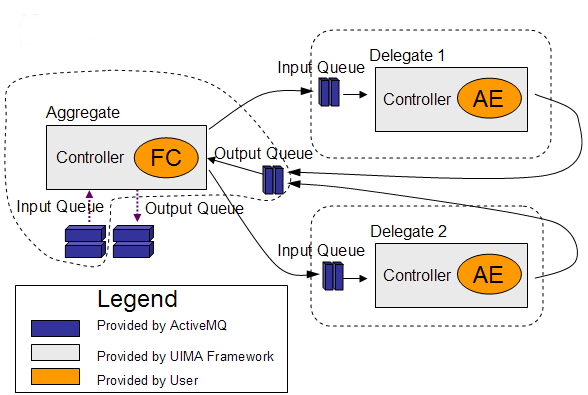
\includegraphics[width=1\textwidth]{uima-as-aea}
	\caption[An aggregate Analysis Engine as a service in UIMA-AS.]{An aggregate Analysis Engine as a service in \uimaas{} \cite{uimaas:documentation}.}
	\label{fig:uimaas-aea}
\end{figure}

Since the \cas{} object contains everything, the \sofa{}, all analysis results, the type system, and maybe even different Views, it can grow quite large over the span of a complicated pipeline. This forms a problem in \uimaas{}, since the \cas{} has to be serialized for every transport inside the system, from client to broker, from broker to service, from Flow Controller to delegate Analysis Engines and the whole way back. Serialization however is a costly task and even if the underlying \nlp{} analysis is very sophisticated, serialization might not be negligible. Epstein et al. handle this problem in \cite{epstein2012making} by avoiding serialization on local instances and introducing a sparse Delta-\cas{} serialization, containing only changes in respect to an original \cas{}.

As most parts of the native \uima{} framework, \uimaas{} is configured by writing an \xml{} descriptor, containing all the necessary data for deployment. A dynamic creation of said descriptor files is currently not possible with \uimafit{}, but is provided by Leo, described in Section~\ref{ssec:leo}.

\section{Distributed Computation}
\label{sec:dist_comp}
When handling large sets of data, a single machine may not be sufficient to solve the given task in a feasible time. In such a scenario, it would be desirable to just add more computation power to finish said task quicker. However, even if the given task permits parallelization, which is not obvious in general, distributing a problem among multiple machines, or similarly processing cores, is not trivial. For many problems a large administrative and communicative overhead aggravates the effort to parallelize.

In this section, some models for parallel and distributed computation are described. Those concepts aim to generalize the problem of distributing a task while at the same time try not to be too restrictive in their interface. 

\subsection{MapReduce}
MapReduce is a programming model for distributed computation of large sets of data on clusters of processing cores and usually multiple machines. Google introduced the MapReduce model in 2003 and used it a few years before announcing 2014 to switch to a less restrictive framework \cite{dean2008mapreduce}.

The MapReduce process consists of three phases, \emph{Map}, \emph{Shuffle}, and \emph{Reduce}. The shuffle phase is usually provided by an implementing framework, both other phases are to be implemented by a user. Let the input data set be $C$, with identifiers $I$. More specifically this means that the following holds:

\[\forall{}c\in{}C:\exists!{}i\in{}I:i\text{ is associated with }c.\]
Furthermore let $K$ be a set of keys and $V$ a set of intermediate values. Then the \lstinline|map| function maps the input data with the associated identifier to a list of key-value pairs:

\[\text{map}:I\times{}C \rightarrow{} (K\times{}V)^*\]
Then the \lstinline|reduce| function reduces a key and a list of all associated intermediate values to a single intermediate value:

\[\text{reduce}: K\times{}V^*\rightarrow{}K\times{}V\]

The \lstinline|reduce| function is often described with a range of just $V$, because it never changes its parameter of $K$ and just passes it through. After all value lists have been reduced to contain only a single value $v\in{}V$, they form the final output $(K\times{}V)^*$.

The canonical example for this model is the problem of counting the number of occurrences for each word in large documents or even larger corpora of documents \cite{dean2008mapreduce}. Recall that for given input documents $C$ and corresponding identifiers $I$, which might be filenames or \URL{}s, one expects a list of key-value pairs containing $k\in{}K$, an identifier for a single word (likely the word itself), and $v\in{}V$ an integer value describing the word's occurrences. Listing~\ref{lst:mapreduce} shows an example implementation of said behavior. Notice that the pseudocode class \lstinline|Word| does refer to a substring containing a single word and not the unit of data.

First, all documents $C$ and their identifying information $I$ are put into $|C|$ instances of the \lstinline|map| function. The results are $|C|$ lists of word-integer pairs. Notice that these intermediate results are not yet distinct. This means that several entries of even the same list might be equal if the corresponding word occurs more than once in one document. Now follows the shuffle operation, which collects intermediate results with the same key on as few machines as possible. This is a costly procedure, since data must be sent over the network. In the third phase, the reduction algorithm gets a word and a number of corresponding counting integers which it just adds and returns. Notice that -- in this example -- the first execution of the \lstinline|reduce| function will receive a word and a list of ones. This is because the \lstinline|map| function initialized each word counter with exactly one.

All intermediate results per word can now be reduced further until only one value remains, which is the final output value. Since the MapReduce model does not define an ordering on the lists given to the \lstinline|reduce| function, it must be associative and commutative to always yield the same result regardless of the inputs ordering. However, MapReduce implementations usually guarantee a fixed ordering to simplify programming the \lstinline|reduce| function.

\begin{lstlisting}[language=Java,caption={Example pseudocode implementation of the MapReduce model to count word occurrences.},label=lst:mapreduce]
List<Pair<Word, Integer>> map(Id docIdentifier, Text docText) {
	List<Pair<Word, Integer>> result = new List<>();
	for(Word w in documentText) {
		result.append((w, 1));
	}
	return result;
}

Pair<Word, Integer> reduce(Word w, List<Integer> intermediate) {
	Integer result = 0;
	for(Integer i in intermediate) {
		result += i;
	}
	return (w, result);
}

\end{lstlisting}
	
Dean and Ghemawat found in \cite{dean2008mapreduce} that many real world applications are describable in the MapReduce model. However, it is still very restrictive and has been abandoned by Google for this very reason. A popular open-source implementation of MapReduce is Apache Hadoop, or more specifically Hadoop MapReduce. It is therefore part of Apache Hadoop, a collection of utilities to handle large amount of data in computation. Apache Hadoop is popular for the \hdfs{}, a high performance distributed file system.

\subsection{Resilient Distributed Datasets}

\rdds{} provide an interface that are very similar to the native Java \lstinline|Collection|. They were initially developed in 2012 by Zaharia et al. in \cite{zaharia2012resilient} as a response to iterative algorithms being inefficient in current computing frameworks such as MapReduce.

An \rdd{} can be created by either of two ways. First, stable data collections such as native Java \lstinline|Collection| instances or a number of files in a file system can be initialized as \rdds{}. The other way of creating is a deterministic operation on an already existing \rdd{}. These operations are called \emph{transformations} by Zaharia in \cite{zaharia2012resilient}. Since \rdds{} are immutable collections, calling such a transformation on an existing \rdd{} is the only way of obtaining the wanted resulting \rdd{}.

Being immutable, \rdds{} allow to be materialized lazily. This means that the issued transformations are executed just in time, when a materialized form of the \rdd{} is necessary. This happens on actions like counting the number of objects in the \rdd{} or serializing it to a file. Before executing these transformations, an acyclic graph is built to represent the necessary transformations of computing said \rdd{}. Furthermore, \rdds{} are sliced into partitions, atomic pieces that never are split in the context of \spark{}. These partitions can then be distributed among the clusters nodes and computed whenever necessary. For the distribution of said partitions, \spark{} utilizes the knowledge of the issued transformation to evaluate dependencies of resulting \rdds{} to their predecessor. This means for example, that a \lstinline|count| operation that follows a large amount of transformations does not necessarily force \spark{} to actually compute all these transformations. For example a transformation \lstinline|crossProduct| on data sets $X$ and $Y$ is guaranteed to result in a collection of size $|X|\cdot{}|Y|$. Materialization of $X\times{}Y$ is not necessary. This technique of lazy transformation provides a simple way of fault tolerance since only the \rdd{} lineage and not the complete materialized \rdd{} itself must be replicated among the different machines.

The only current implementation of \rdds{} is Apache \spark{}, introduced along with \rdds{} in 2012 \cite{zaharia2012resilient}.

\section{Containerization and Docker}
Containerization describes the virtualization of applications while using the existing host kernel. This distinguishes containerization from using a \vm{}. A \vm{} simulates a completely different hardware stack than the hosts and provides a full kernel. This makes it possible to run a virtual machine with an operating system different from that the host has and provides a near perfect isolation of host and guest.

This is different from a container inside a host operating system. Since one kernel is shared, a container can only use the host's system calls and hardware. This makes containers more light-weight than \vms{} but also less flexible in terms of the host operating system. There are also concerns about security since the isolation layer between host and guest is thinner and a guest might break out easier than in a \vm{} \cite{turnbull2014docker,jian2017defense}.

\docker{} is such a containerization tool that was first released in 2013 by Docker, Inc. A \docker{} container is instantiated by an \emph{image}. An image specifies the exact user space inside the starting container and is usually defined by taking a base image and installing necessary libraries or programs for the containerized application to launch. Listing~\ref{lst:uimaas} shows a Dockerfile, an exact definition of how instantiated containers of the resulting image will be configured.
\begin{lstlisting}[caption={An example Dockerfile for an UIMA-AS image.},label=lst:uimaas,morekeywords={FROM,ADD,RUN,ENV,EXPOSE}]
	FROM openjdk:8
	
	# Install UIMA-AS.
	ADD uima-as-2.10.2-bin.tar.gz /uima-as
	RUN mv /uima-as/apache-uima-as-2.10.2/* /uima-as
	RUN rm -rf /uima-as/apache-uima-as-2.10.2
	RUN mkdir /uima-as/classpath
	
	# Set environment variables.
	ENV UIMA_HOME=/uima-as
	ENV PATH="/uima-as/bin:${PATH}"
	ENV ACTIVEMQ_BASE=/active-mq
	ENV UIMA_CLASSPATH=/uima-as/classpath
	
	# Expose necessary ports.
	EXPOSE 61616
	EXPOSE 8080
\end{lstlisting}
First, the base image is defined. Here, the official image for openJDK for Java 8 was used, a slim image containing a working openJDK installation and nothing else. Next, \uimaas{} is installed, provided that the corresponding TAR file is available at the current folder. It is first added to the image and unpacked in the same step. Then the folder's name is changed in order to omit the version number. Afterwards a directory is created to function as appendix to \uimaas{}' classpath. Every JAR and CLASS file in this folder will be loaded into an \uimaas{} instance. Without the use of simplifying frameworks like Leo (Section~\ref{ssec:leo}), Analysis Engines must be available to \uimaas{}' classpath.

After successful installation of \uimaas{}, some environment variables must be set and the \lstinline|PATH| variable must be modified. This is possible by the \lstinline[morekeywords={ENV}]|ENV| command as shown in Listing~\ref{lst:uimaas}. At last, the ports that this image exposes must be defined. Since \uimaas{} transfers data via the Java Messaging Server over 61616 or HTTP over 8080, both ports must be exposed. Notice that both ports are configurable inside the \uimaas{} configuration files. However, since port remapping is easily done in the docker composition and nothing else should ever run inside the dedicated \uimaas{} container, reconfiguration of the default ports is usually discouraged.

After building the image defined in Listing~\ref{lst:uimaas}, one might use it to start containers or push it to repositories. Notice that multiple instances of this image may be run simultaneously on the same machine. To enable access to every instance and allow inter-container connections, a configuration file can be utilized to create what is called a \emph{\docker{} composition}. This defines how different containers may communicate with each other and how running instances depend on other containers. An important feature for the evaluation in Chapter~\ref{ch:evaluation} is the limitation of hardware resources available in composition configuration files.

\docker{} and any other form of containerization were not used for the framework presented in Chapter~\ref{ch:implementation}. However, it was heavily utilized to simulate networks and multiple machines in Chapter~\ref{ch:evaluation}.

\section{Related Work}
\label{sec:related}
Taking effort to scale \uima{} has been done numerous times. The most prominent result was the implementation of the question answering system Watson \cite{epstein2012making}. This approach used native \uimaas{}, although the engineers changed the \uimaas{} source code themselves. Other approaches that are trying to be generic solutions while not posing too many restrictions or being too intrusive into the native \uima{} concepts or even code, are Leo and v3NLP.

\subsection{Leo}
\label{ssec:leo}
The Leo framework was developed by \vinci{} to allow for the easy deployment of annotators in an \uimaas{} environment \cite{leo}. Since it wraps around most concepts of \uima{} and \uimaas{}, its architecture closely resembles \uimaas{}. This can be seen in Figure~\ref{fig:leo}. Given a number of instances of \lstinline|LeoAEDescriptor|, which are compatible with the native \uima{} Analysis Engine, Leo is able to automatically write an \uimaas{} deployment descriptor file and use it to deploy a \lstinline|Service| instance. This also is just a wrapper around \uimaas{} native service, which tries to register to a given broker implementation. Leo does not provide a broker implementation by its own, but depends on an existing \uimaas{} installation, which in turn provides ActiveMQ, as described further in Section~\ref{ssec:uimaas}.
\begin{figure}[hbt]
	\centering
	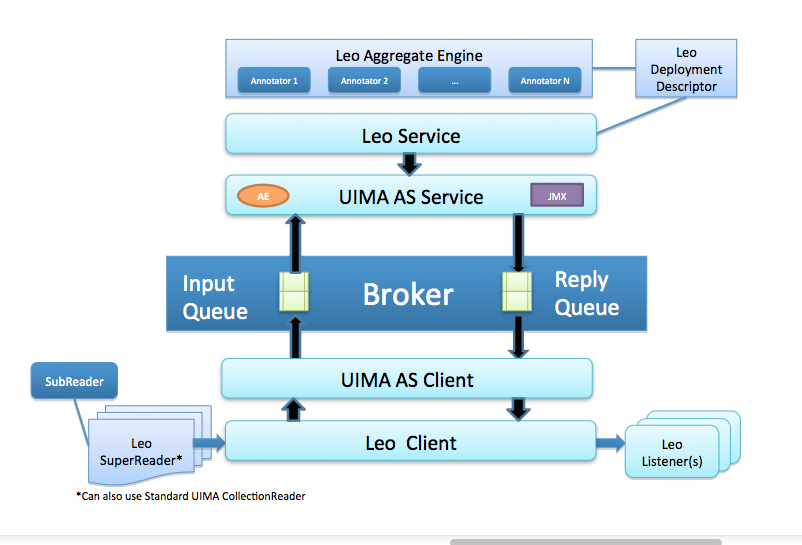
\includegraphics[width=1\textwidth]{leo}
	\caption[The Leo architecture wrapping around UIMA-AS.]{The Leo architecture wrapping around \uimaas{} \cite{leo}}
	\label{fig:leo}
\end{figure}
Given such an instance of a broker-service architecture, Leo is now able to perform requests to said broker. The Leo \lstinline|Client| class provides access to the native \uimaas{} capability of querying the services for analysis results. For this, Leo utilizes the class \lstinline|LeoCollectionReader|, which also is just a wrapper around the native \uima{} Collection Readers and can be easily converted to one and vice versa.

The Leo source code repository\footurl{https://github.com/department-of-veterans-affairs/Leo}{2018-09-14} shows that the last change was in January 2018, without providing any comments or history\footurl{https://github.com/department-of-veterans-affairs/Leo/commit/038f7d5c542fa564c2997403769943ac47638692}{2018-09-14}. This, and the fact that the project only has four contributors and no pull request as of the time of writing shows that the Leo framework project is not well-maintained.

A static code analysis with FindBugs\footurl{http://findbugs.sourceforge.net/}{2018-09-14} on the current source code\footnote{Commit 038f7d5c542fa564c2997403769943ac47638692 on 2018-09-14} shows 29 potential bugs, of which seven are rated as `scary' by FindBugs. Another code analysis tool, SonarLint\footurl{https://www.sonarlint.org/}{2018-09-14} which also checks the coding style found a total of 626 bugs, vulnerabilities and code smells. 

\subsection{v3NLP}
The framework v3NLP was first introduced in 2011 by Divita and Trietler in \cite{divita2011finding} as a successor to HITEx\footnote{Health Information Text Extraction}. Both, HITEx and v3NLP were initially built on top of the Gate framework but have switched to \uima{} since. v3NLP provides capabilities to process \nlp{} tasks especially in the medical field. It is therefore heavily influenced by the context of a medical environment. It provides 34 pre-composed pipelines, all related to clinical text analysis. However, it enforces the use of the CHIR\footnote{Consortium for Healthcare Informatics Research} Common Model, which is an ontology of labels from already existing \nlp{} systems. This model is encoded in a default type system the framework is using and it can be extended at will. This is supposed to ensure interoperability between different \nlp{} components that were developed for v3NLP. Notice that this poses a restriction on the user of the framework, since they are forced to always include this type system \cite{divita2016v3nlp}. The framework also provides scaling capabilities that internally utilize the native \uimaas{} scalability.

While the v3NLP framework provides many functionalities for \nlp{} research in the medical context, it is a large project in respect to \uima{}, \uimaas{} and Leo (described in Section~\ref{ssec:leo}). All the v3NLP git repositories combined span 23.3\,GB of content and contain about 1.8\,million lines of Java code in the latest commit alone. Thus it is a heavyweight tool, which is used best in a medical environment where as many capabilities as possible are actually used.

At the time of writing, the last commit to the framework repository was on December 2017, nine months in the past. According to the v3NLP website\footurl{http://inlp.bmi.utah.edu/redmine/docs/v3nlp-framework/News.html}{2018-09-14} this is expected to be the very last commit.




%In this chapter, we will cover the basics for the necessary technologies used throughout the evaluation. All of these are concrete implementations of more general concepts and may be exchanged for similar products. However, the following products were chosen, mainly because they are Open Source\footurl{https://svn.apache.org/viewvc/uima/}{2018-02-27}\footurl{https://github.com/docker}{2018-02-27}\footurl{https://github.com/apache/hadoop}{2018-02-27}\footurl{https://github.com/apache/spark}{2018-02-27}\footurl{https://github.com/apache/kafka}{2018-02-27} but also because of their popularity and relevance in the industry.

% % !TeX root = ../Main.tex

\section{UIMA}
\uima{} is a data mining and \nlp{} framework, created in 2005 by IBM \cite{ferrucci2004uima} and maintained by Apache since 2006 \cite{uimacpe}. It is available in Java and C++ and contains various scale-out options. 
Strictly speaking, one has to differentiate between the \uima{} specification and Apache \uima{}, an open source implementation of said specification \cite{OASIS:UIMA:2009}. Since both terms are often used interchangeably, this thesis will also not differentiate between Apache \uima{} and \uima{}. Unless specified else, we will always reference the Apache \uima{} implementation.

\marginnote{Alles ein wenig wirr. Braucht rewrite. Weiß aber nicht genau wie tief in die Materie ich hier gehen muss.}
The \uima{} specification describes \nlp{} applications as a collection of (mostly) independent components. Such a component is called an \anen{} and enriches a given document by inferred information. To modularize said components, \uima{} provides the notion of a \cas{}. A \cas{} is an object containing the \sofa{}, the analysis results and the used type system.



% % !TeX root = ../Main.tex

\section{\docker{}}
\marginnote{Source?}\docker{} is a software to create and run applications in virtual environments, without the need to setup a complete virtual operating system for each application. Based on Cgroups and namespaces, \docker{} runs applications in a containerized environment.
To create a containerized application, a special markup file, called a Dockerfile has to be written by the programmer. The Dockerfile defines exactly how the applications' environment needs to look like. Listing \ref{dockerfile} shows how such a Dockerfile typically looks like. Based on an Ubuntu image, it installs Java via apt-get. Afterwards it copies the file {\em{} application.jar} into the root of the image and tells \docker{} to execute it via \lstinline[]|java -jar /app.jar -Xmx4G -Xms4G|. Having such a Dockerfile ensures reproducibility of the constructed images. After building said Dockerfile, an image is created.\marginnote{source für Registries? Öffentliches \docker{}-Registry?} This image can be serialized into a file but is usually uploaded to \docker{} repositories, called registries. 

\begin{minipage}{\textwidth}
	
\begin{lstlisting}[style=YAML,caption=A sample Dockerfile used for creating a simple Ubuntu based image to start a Java application.,label=dockerfile]
FROM	ubuntu

RUN		apt(*@-@*)get update
RUN		apt(*@-@*)get install openjdk(*@-@*)9(*@-@*)jre

COPY	./application.jar /application.jar

ENTRYPOINT ["java", "(*@-@*)jar /app.jar", "(*@-@*)Xmx4G", "(*@-@*)Xms4G"]
\end{lstlisting}

\end{minipage}

\marginnote{SOUUUURCE!!}If published through a registry, \docker{} automatically downloads images on demand. Since the application as well as the whole environment necessary to run it lie within the image, it can be executed. \docker{} creates a container, a virtual environment based on the given image, \marginnote{Zweimal within? Thesaurus lässt grüßen.}and runs the application within. Containers are usually not aware of each other, thus the same application can be started multiple times, just by starting more containers. \marginnote{An den Haaren herbeigezogen.}This modular view on containers will play a fundamental role on scaling.
% % !TeX root = ../Main.tex

\section{Hadoop}
\marginnote{Sauce!}\hadoop{} is an open-source framework for computation and storage, distributed over an \marginnote{almost?}(almost) arbitrary number of machines. It contains the \hdfs{}, a distributed file system built for high throughput and reliability, and specifically designed to run on commodity hardware. These properties allow for large clusters of relatively cheap hardware.

\hadoop{} also provides an API for distributed computing, named Hadoop MapReduce, based on the MapReduce algorithm by Dean and Ghemawat in \cite{dean2008mapreduce}. In this algorithm the underlying transformation of data is abstracted into two general steps, Map and Reduce. With $K,L,V,W$ being sets the Map function implements 
\[\mathtt{Map}: K\times{}V\to{}(L\times{}W)^*\]
Thus it maps a key-value pair to a list of key-value pairs of arbitrary length \cite{wiki:mapreduce}. The resulting list of key-value pairs acts as intermediate values. The Reduce function aggregates those intermediate values with
\[\mathtt{Reduce}: L\times{}W^*\to{}\] huh...
The programmer in question needs to understand this concept and divide their code into those two steps.
% \section{Spark}
% \section{Kafka}
